\documentclass{article}

\usepackage{fullpage}
\usepackage{graphicx}
\usepackage{subfig}
\usepackage[colorlinks, linkcolor=blue]{hyperref}

\newcommand{\tbbmap}{\texttt{concurrent\textunderscore hash\textunderscore map}}
\newcommand{\libcuckoo}{\texttt{libcuckoo}}

\title{Comparing Intel TBB {\tbbmap} and \libcuckoo}
\author{Manu Goyal, Dave Andersen, Michael Kaminsky}
\date{\today}

\begin{document}

\maketitle{}

\section*{Overview}

In this benchmark, we compare {\libcuckoo}, our high-performance,
memory-efficient hash table, with the Intel Thread Building Blocks {\tbbmap}
version 4.4. We compare the performance of the two tables across different types
of workloads and different numbers of cores, and also compare the memory usage
for different table sizes. We ran the benchmarks on a machine with 36 Intel Xeon
2.9 GHz cores and 60GB memory. The cores were split evenly into two NUMA nodes.

The benchmarks we ran measure pure read, pure insert, and mixed read-insert
performance, as well as peak memory usage. For the performance benchmarks, we
benchmarked maps with 64-bit integer keys, randomly shuffled numbers in the
range 0 to the capacity of the table, as well as maps with 100-character string
keys, designed to maximize comparison time.

\section*{Pure Read}
Our read benchmark fills a table up to 90\% of its allocated capacity, then
concurrently runs reads for data that is in the table and data that isn't. It
counts the number of reads executed over 10 seconds. Figure~\ref{fig:pure-read}
compares the read throughput of the two tables with integer and string keys. For
both types of keys, {\libcuckoo} outperforms {\tbbmap}, with the difference
getting slightly larger as we increase the number of threads. With 32 threads,
{\libcuckoo} outperforms {\tbbmap} by 47\% for integers, and 37\% for string
keys.

\begin{figure}[!htbp]
  \centering
  \subfloat[]{{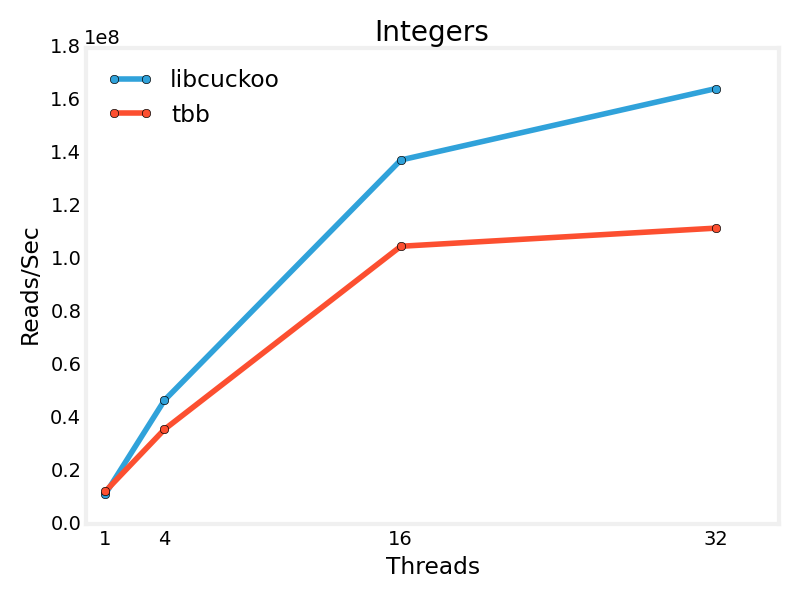
\includegraphics[width=0.5\textwidth]{read-integer}}}
  \subfloat[]{{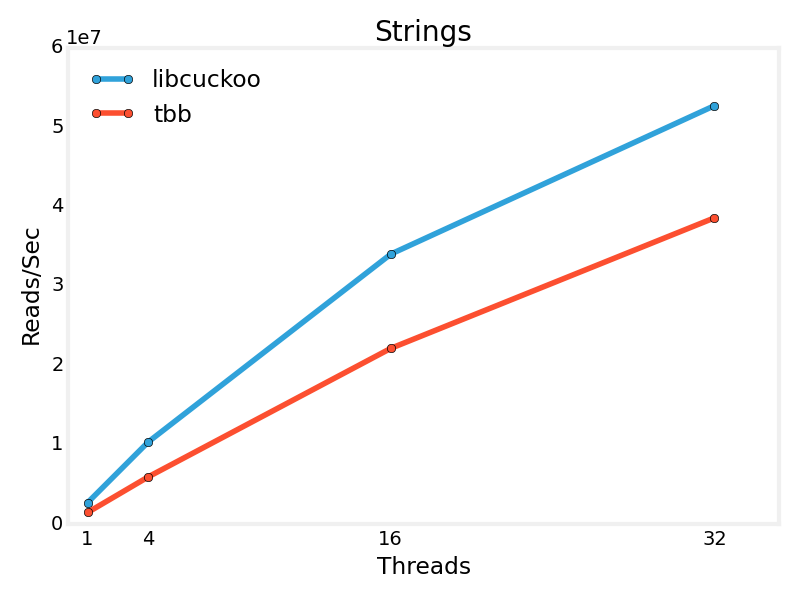
\includegraphics[width=0.5\textwidth]{read-string}}}
  \caption{Pure read throughput for integer and string keys}
  \label{fig:pure-read}
\end{figure}

\section*{Pure Insert}
Our insert benchmark measures the time taken to fill up a table from 0\% to 90\%
of its allocated capacity. Figure~\ref{fig:pure-insert} compares the insert
throughput with integer and string keys. For integers, {\libcuckoo} greatly
outperforms {\tbbmap}, by over 680\%, and for strings, it outperforms {\tbbmap}
by 50\%. It is interesting to note that {\tbbmap}'s performance actually drops
when we go from 4 threads to 16 threads, and then increases only slightly when
we go up to 32 threads. With strings, since the cost of copying strings likely
dominates the runtime, this effect is less apparent.

We suspect that part of the reason for this poor scaling is due to the fact that
{\tbbmap} doesn't deal well with multiple NUMA clusters, because data tends to
be modified by CPUs on different NUMA clusters. {\libcuckoo} specifically avoids
this issue by separating all shared data by core, so minimal data ends up being
transferred across NUMA nodes. Figure~\ref{fig:pure-insert-one-numa} confirms
this hypothesis. {\tbbmap} increases its throughput by over 240\% on 16 threads,
compared to its performance in Figure~\ref{fig:pure-insert}, while {\libcuckoo}
is not much affected by restricting to one NUMA node, increasing throughput by a
more modest 26\%. In both cases, {\libcuckoo} significantly outperforms
{\tbbmap} on integer inserts.

Another possibility for the performance difference is the data cache or TLB miss
rate. We roughly examined these numbers for both tables, and found that the
cache miss rate was about the same for both tables, with {\libcuckoo} tending to
be slightly lower. The TLB miss rate, however, was far higher for {\tbbmap},
likely due to the larger memory footprint. We mitigated this problem by
utilizing linux hugepages in {\tbbmap}, and, while this did decrease the TLB
miss rate of {\tbbmap} significantly, it had no effect on performance. So
ultimately, cache and TLB miss rates do not seem to explain the performance
difference for inserts.

\begin{figure}[!htbp]
  \centering
  \subfloat[]{{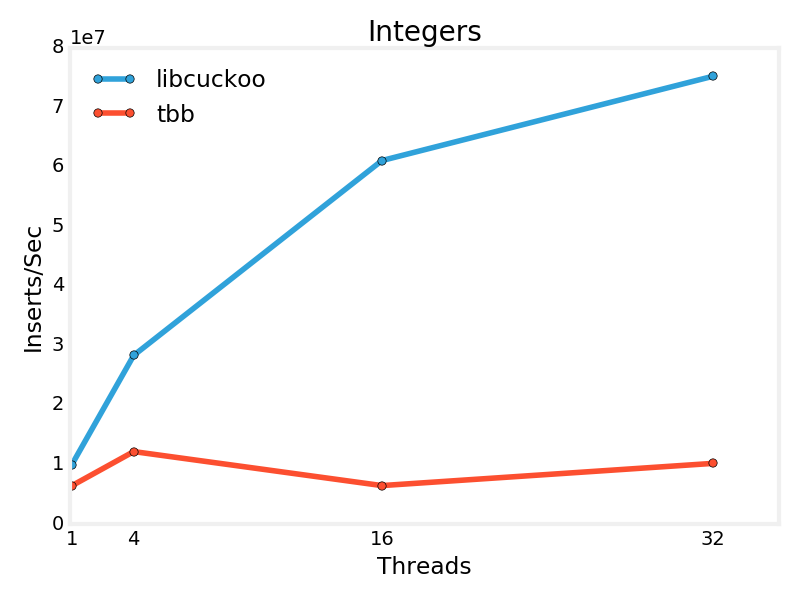
\includegraphics[width=0.5\textwidth]{insert-integer}}}
  \subfloat[]{{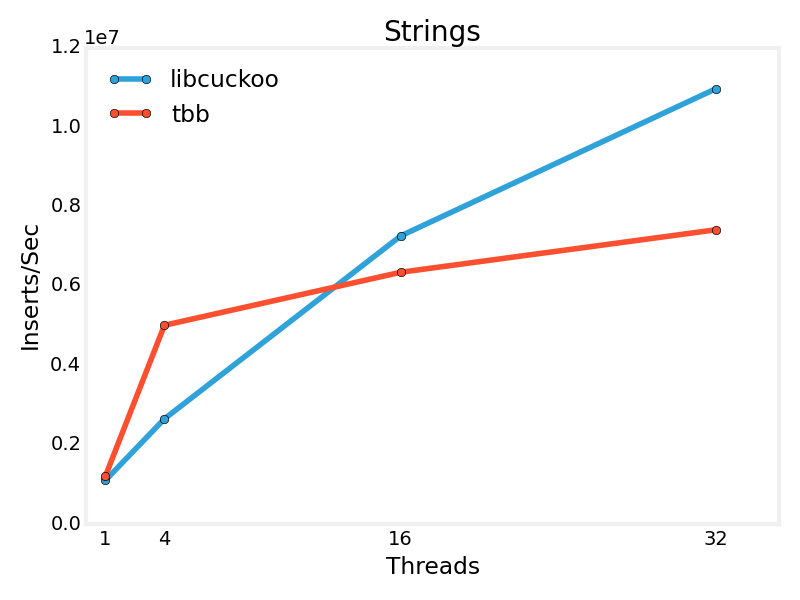
\includegraphics[width=0.5\textwidth]{insert-string}}}
  \caption{Pure insert throughput for integer and string keys}
  \label{fig:pure-insert}
\end{figure}

\begin{figure}[!htbp]
  \centering
  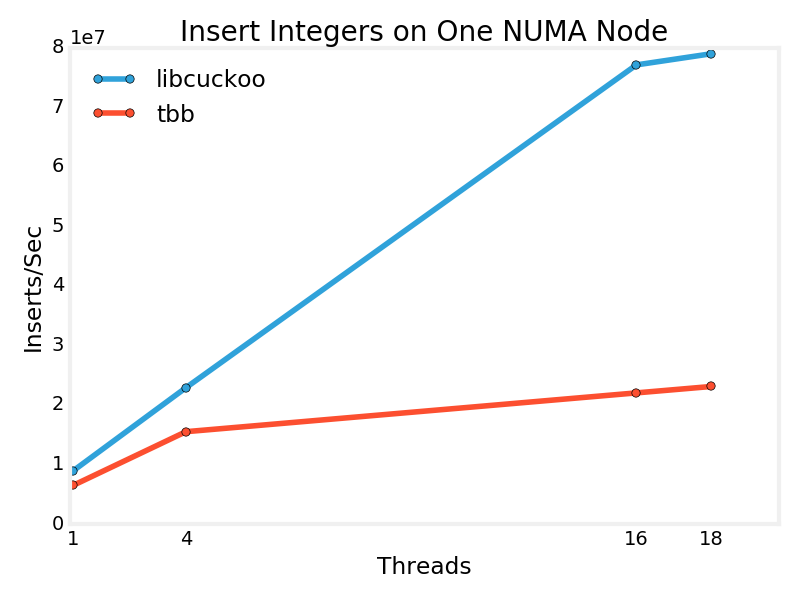
\includegraphics[width=0.5\textwidth]{insert-integer-one-numa}
  \caption{Pure insert  for integer and string keys on one NUMA node}
  \label{fig:pure-insert-one-numa}
\end{figure}

\section*{Mixed Workload}
Our mixed benchmark runs a mixed workload of inserts and reads at a configurable
ratio, and measures the time and number of operations taken to fill up the table
from 0\% to 90\% of its allocated capacity. Figure~\ref{fig:mixed-read-insert}
compares the performance of the two tables at different ratios of inserts (all
with 32 threads), with {\libcuckoo} doing better with both integer and string
keys. We see again that the difference between the two tables is much greater at
higher insert percentages compared to lower percentages (588\% compared to 36\%,
respectively), because the difference between {\libcuckoo} and {\tbbmap} is more
pronounced for inserts than it is for reads.

\begin{figure}[!htbp]
  \centering
  \subfloat[]{{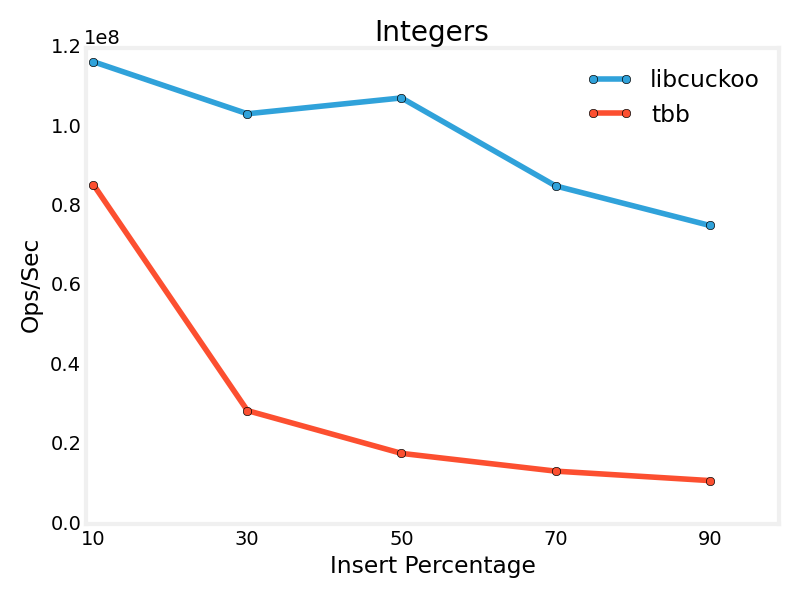
\includegraphics[width=0.5\textwidth]{read-insert-integer}}}
  \subfloat[]{{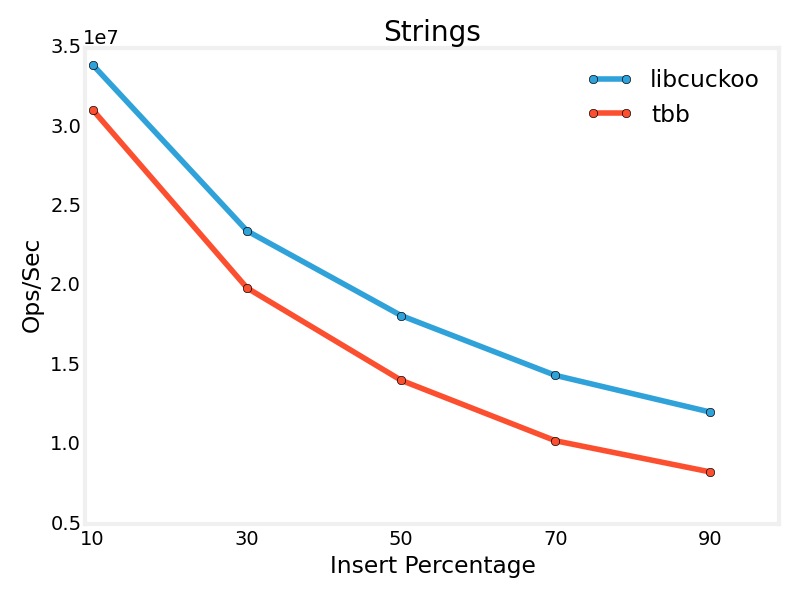
\includegraphics[width=0.5\textwidth]{read-insert-string}}}
  \caption{Mixed read-insert throughput for integer and string keys}
  \label{fig:mixed-read-insert}
\end{figure}

\section*{Memory Usage}
Finally, we compare the approximate memory usage of the two tables. While not a
completely accurate measure of the amount of memory used by each table, we
measured the maximum resident set size as determined by Ubuntu's \texttt{time}
command for the insert benchmark, which is the peak memory usage for the
process. For integers, {\libcuckoo} scales far better than {\tbbmap}, using 72\%
less memory than {\tbbmap} with the largest table.

\begin{figure}[!htbp]
  \centering
  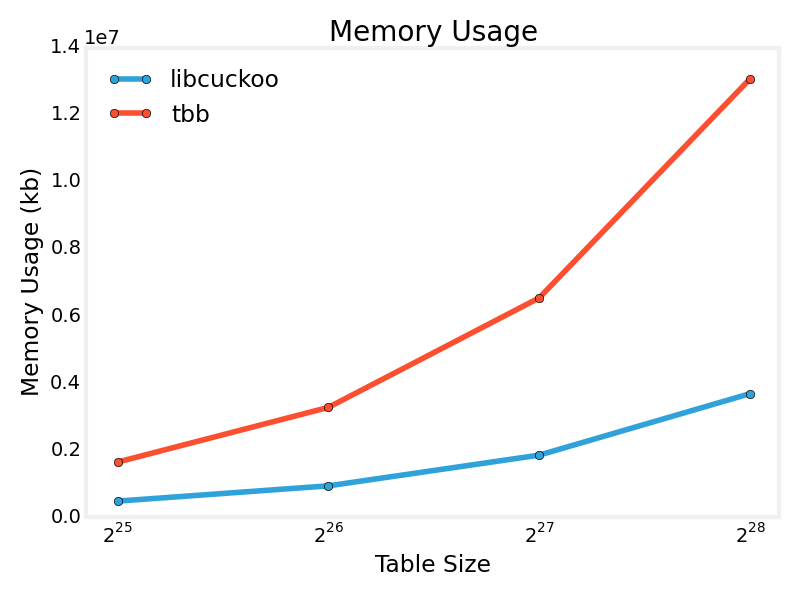
\includegraphics[width=0.5\textwidth]{mem}
  \caption{Peak memory usage for insert benchmark with integer keys. Table size
    is the number of elements each table has capacity for}
  \label{fig:mem}
\end{figure}

\section*{Conclusion}

{\libcuckoo} has a number of features that cause it to perform better and use
less memory than {\tbbmap}. {\libcuckoo} stores data in a cache-optimized form
and avoids false sharing between CPU's, which allow it to scale inserts and
reads very well to a large number of CPU's with low memory overhead.
Furthermore, the cuckoo hashing algorithm lets it achieve very high table load
factors before needing to expand, which significantly reduces memory usage.

\end{document}

%%% Local Variables:
%%% mode: latex
%%% TeX-master: t
%%% End:
